% ====================================================================
%  徐森林、金亚东、薛春华《数学分析》（第三册）
%  第 16 章  Fourier 分析
%  §16.1  周期函数的 Fourier 级数及收敛定理 (PART-A)
%  源：原书印刷页 244-256（PDF 物理页 250-262）
% ====================================================================

\section{周期函数的 Fourier 级数及收敛定理}\label{sec:16.1}

设 $g(t)$ 是以 $T\neq 0$ 为周期的周期函数, 即 $g(t+T)=g(t)$, 作变量代换
\[
  x=\frac{2\pi}{T}t\quad\text{或}\quad t=\frac{T}{2\pi}x,
\]
就有
\[
  g(t)=g\left(\frac{T}{2\pi}x\right)=f(x).
\]
于是, $f(x)$ 就是以 $2\pi$ 为周期的周期函数. 因此, 只需讨论以 $2\pi$ 为周期的周期函数. 设 $f(x)$ 是以 $2\pi$ 为周期的周期函数, 自然会问, 在什么条件下, $f(x)$ 能表示为
\[
  f(x)=\frac{a_{0}}{2}+\sum_{n=1}^{\infty}(a_{n}\cos nx+b_{n}\sin nx).
\]
此外, 如何确定系数 $a_{0}, a_{n}, b_{n}$ ($n=1,2,\cdots$).

\begin{theorem}\label{thm:16.1.1}
设以 $2\pi$ 为周期的周期函数 $f(x)$ 可表示为
\[
  f(x)=\frac{a_{0}}{2}+\sum_{n=1}^{\infty}(a_{n}\cos nx+b_{n}\sin nx).
\]
如果上述级数在 $[-\pi,\pi]$ 上一致收敛于 $f(x)$, 则
\[
  \left\{\begin{aligned}
    a_{n}&=\frac{1}{\pi}\int_{-\pi}^{\pi}f(x)\cos nx\,\mathrm{d}x,\quad n=0,1,2,\cdots,\\
    b_{n}&=\frac{1}{\pi}\int_{-\pi}^{\pi}f(x)\sin nx\,\mathrm{d}x,\quad n=1,2,\cdots.
  \end{aligned}\right.
\]
\end{theorem}

\begin{proof}
因为 $\displaystyle\frac{a_{0}}{2}+\sum_{n=1}^{\infty}(a_{n}\cos nx+b_{n}\sin nx)$ 在 $[-\pi,\pi]$ 上一致收敛于 $f(x)$, 根据函数项级数一致收敛的 Cauchy 准则知,
\[
  \frac{a_{0}}{2}\cos nx+\sum_{k=1}^{\infty}(a_{k}\cos kx\cos nx+b_{k}\sin kx\cos nx)
\]
在 $[-\pi,\pi]$ 上一致收敛于 $f(x)\cos nx$. 应用逐项积分的定理~\ref{thm:13.2.3p}得到
\[
  \begin{aligned}
    \int_{-\pi}^{\pi}f(x)\cos nx\,\mathrm{d}x&=\frac{a_{0}}{2}\int_{-\pi}^{\pi}\cos nx\,\mathrm{d}x\\
    &\quad+\sum_{k=1}^{\infty}\left(a_{k}\int_{-\pi}^{\pi}\cos kx\cos nx\,\mathrm{d}x+b_{k}\int_{-\pi}^{\pi}\sin kx\cos nx\,\mathrm{d}x\right)\\
    &\xlongequal{\text{\extref{例 6.3.3}}}\frac{a_{0}}{2}\cdot 2\pi\delta_{0n}+\sum_{k=1}^{\infty}(a_{k}\cdot\pi\delta_{kn}+b_{k}\cdot 0)=\pi a_{n},\quad n=0,1,2,\cdots,
  \end{aligned}
\]
其中
\[
  \delta_{kn}=\begin{cases}
    1, & k=n,\\
    0, & k\neq n.
\end{cases}
\]
同理, 有
\[
  \begin{aligned}
    \int_{-\pi}^{\pi}f(x)\sin nx\,\mathrm{d}x&=\frac{a_{0}}{2}\int_{-\pi}^{\pi}\sin nx\,\mathrm{d}x\\
    &\quad+\sum_{k=1}^{\infty}\left(a_{k}\int_{-\pi}^{\pi}\cos kx\sin nx\,\mathrm{d}x+b_{k}\int_{-\pi}^{\pi}\sin kx\sin nx\,\mathrm{d}x\right)\\
    &\xlongequal{\text{\extref{例 6.3.3}}}\frac{a_{0}}{2}\cdot 0+\sum_{k=1}^{\infty}(a_{k}\cdot 0+b_{k}\cdot\pi\delta_{kn})=\pi b_{n},\quad n=1,2,\cdots.
  \end{aligned}
\]
于是得到
\[
  \left\{\begin{aligned}
    a_{n}&=\frac{1}{\pi}\int_{-\pi}^{\pi}f(x)\cos nx\,\mathrm{d}x,\quad n=0,1,2,\cdots,\\
    b_{n}&=\frac{1}{\pi}\int_{-\pi}^{\pi}f(x)\sin nx\,\mathrm{d}x,\quad n=1,2,\cdots.
  \end{aligned}\right.
\]
\end{proof}

\begin{definition}\label{def:16.1.1}
设 $f(x)$ 是周期为 $2\pi$ 的函数, 它在 $[-\pi,\pi]$ 上可积或绝对可积 (如果 $f(x)$ 是有界函数, 就假定它是 Riemann 可积的, 简称可积; 如果 $f(x)$ 是无界函数, 就假定它是广义绝对可积的, 简称绝对可积). 称由公式
\[
  \left\{\begin{aligned}
    a_{n}&=\frac{1}{\pi}\int_{-\pi}^{\pi}f(x)\cos nx\,\mathrm{d}x,\quad n=0,1,2,\cdots,\\
    b_{n}&=\frac{1}{\pi}\int_{-\pi}^{\pi}f(x)\sin nx\,\mathrm{d}x,\quad n=1,2,\cdots
  \end{aligned}\right.
\]
确定的 $a_{n}, b_{n}$ 为 $f(x)$ 的 \textbf{Fourier 系数}, 由 $a_{n}, b_{n}$ 确定的级数
\[
  \frac{a_{0}}{2}+\sum_{n=1}^{\infty}(a_{n}\cos nx+b_{n}\sin nx)
\]
称为 $f(x)$ 的 \textbf{Fourier 级数}, 记为
\[
  f(x)\sim\frac{a_{0}}{2}+\sum_{n=1}^{\infty}(a_{n}\cos nx+b_{n}\sin nx).
\]
\end{definition}

至于这个级数是否收敛, 如果收敛的话, 它的和是否就等于 $f(x)$, 这些问题都有待进一步研究. 但有一点是可以肯定的, 这个级数是由 $f(x)$ 确定的.

在推论~\ref{cor:16.1.3}中将看到, 对于相当广泛的一类函数, 它的 Fourier 级数是收敛于它自己的, 这正是 Fourier 级数所以重要的原因.

\begin{theorem}[Riemann-Lebesgue 引理]\label{thm:16.1.2}
设 $f(x)$ 在 $[a,b]$ 上可积或绝对可积, 则
\[
  \lim_{\lambda\to+\infty}\int_{a}^{b}f(x)\cos\lambda x\,\mathrm{d}x=0,\quad \lim_{\lambda\to+\infty}\int_{a}^{b}f(x)\sin\lambda x\,\mathrm{d}x=0.
\]
\end{theorem}

\begin{proof}
只证第一个等式, 第二个等式的证明完全类似.

\textbf{情形 1: $f(x)$ 在 $[a,b]$ 上有连续导数.}

此时, 应用分部积分公式, 有
\[
  \begin{aligned}
    \left|\int_{a}^{b}f(x)\cos\lambda x\,\mathrm{d}x\right|&=\left|\frac{1}{\lambda}\left(\left.f(x)\sin\lambda x\right|_{a}^{b}-\int_{a}^{b}f'(x)\sin\lambda x\,\mathrm{d}x\right)\right|\\
    &\leqslant\frac{1}{\lambda}\left(|f(b)|+|f(a)|+\int_{a}^{b}|f'(x)|\,\mathrm{d}x\right)\to 0\quad(\lambda\to+\infty).
  \end{aligned}
\]

\textbf{情形 2: $f(x)$ 在 $[a,b]$ 上可积.}

由\extref{定理 6.2.2}知, $\forall\varepsilon>0$, 存在连续函数 $g(x)$, 使得
\[
  \int_{a}^{b}|f(x)-g(x)|\,\mathrm{d}x<\frac{\varepsilon}{3}.
\]
再由 Weierstrass 多项式逼近定理 (\extref{定理 13.2.8}) 知, 存在多项式 $P(x)$, 使得
\[
  \max_{x\in[a,b]}|g(x)-P(x)|<\frac{\varepsilon}{3(b-a)}.
\]
于是,
\[
  \int_{a}^{b}|g(x)-P(x)|\,\mathrm{d}x<\frac{\varepsilon}{3}.
\]
由情形 1 知, 存在 $\Lambda>0$, 当 $\lambda>\Lambda$ 时,
\[
  \left|\int_{a}^{b}P(x)\cos\lambda x\,\mathrm{d}x\right|<\frac{\varepsilon}{3}.
\]
因此, 当 $\lambda>\Lambda$ 时,
\[
  \begin{aligned}
    \left|\int_{a}^{b}f(x)\cos\lambda x\,\mathrm{d}x\right|&\leqslant\int_{a}^{b}|f(x)-g(x)|\,\mathrm{d}x+\int_{a}^{b}|g(x)-P(x)|\,\mathrm{d}x+\left|\int_{a}^{b}P(x)\cos\lambda x\,\mathrm{d}x\right|\\
    &<\frac{\varepsilon}{3}+\frac{\varepsilon}{3}+\frac{\varepsilon}{3}=\varepsilon.
  \end{aligned}
\]

\textbf{情形 3: $f(x)$ 在 $[a,b]$ 上绝对可积.}

假定无界点在端点 $a$ (对于有限个无界点, 或无界点在区间内部的情形, 可分段化为此种情形). 由广义绝对可积的定义知, $\forall\varepsilon>0$, 存在 $a'>a$, 使得
\[
  \int_{a}^{a'}|f(x)|\,\mathrm{d}x<\frac{\varepsilon}{2}.
\]
因为 $f(x)$ 在 $[a',b]$ 上可积, 由情形 2 知, 存在 $\Lambda>0$, 当 $\lambda>\Lambda$ 时,
\[
  \left|\int_{a'}^{b}f(x)\cos\lambda x\,\mathrm{d}x\right|<\frac{\varepsilon}{2}.
\]
从而, 当 $\lambda>\Lambda$ 时,
\[
  \left|\int_{a}^{b}f(x)\cos\lambda x\,\mathrm{d}x\right|\leqslant\int_{a}^{a'}|f(x)|\,\mathrm{d}x+\left|\int_{a'}^{b}f(x)\cos\lambda x\,\mathrm{d}x\right|<\frac{\varepsilon}{2}+\frac{\varepsilon}{2}=\varepsilon.
\]
\end{proof}

\begin{theorem}\label{thm:16.1.3}
设 $\{a_{n}\}, \{b_{n}\}$ 为可积或绝对可积函数的 Fourier 系数序列, 则
\[
  \lim_{n\to+\infty}a_{n}=0,\quad \lim_{n\to+\infty}b_{n}=0.
\]
\end{theorem}

\begin{proof}
直接由定理~\ref{thm:16.1.2} (取 $[a,b]=[-\pi,\pi]$, $\lambda=n$) 即得.
\end{proof}

\begin{remark}\label{rem:16.1.1}
如果 $\lim\limits_{n\to+\infty}a_{n}\neq 0$ 或 $\lim\limits_{n\to+\infty}b_{n}\neq 0$, 则三角级数 $\displaystyle\frac{a_{0}}{2}+\sum_{n=1}^{\infty}(a_{n}\cos nx+b_{n}\sin nx)$ 一定不是任何可积或绝对可积函数的 Fourier 级数.
\end{remark}

\begin{theorem}\label{thm:16.1.4}
设 $f(x)$ 在 $[-\pi,\pi]$ 上连续, $f(-\pi)=f(\pi)$, 且有可积或绝对可积的导函数 $f'(x)$, 则
\[
  a_{n}=o\left(\frac{1}{n}\right),\quad b_{n}=o\left(\frac{1}{n}\right)\quad(n\to+\infty).
\]
\end{theorem}

\begin{proof}
应用分部积分公式,
\[
  \begin{aligned}
    a_{n}&=\frac{1}{\pi}\int_{-\pi}^{\pi}f(x)\cos nx\,\mathrm{d}x=\frac{1}{n\pi}\left(\left.f(x)\sin nx\right|_{-\pi}^{\pi}-\int_{-\pi}^{\pi}f'(x)\sin nx\,\mathrm{d}x\right)\\
    &=-\frac{1}{n\pi}\int_{-\pi}^{\pi}f'(x)\sin nx\,\mathrm{d}x.
  \end{aligned}
\]
由定理~\ref{thm:16.1.2}知, $\lim\limits_{n\to+\infty}\displaystyle\frac{1}{\pi}\int_{-\pi}^{\pi}f'(x)\sin nx\,\mathrm{d}x=0$, 故 $a_{n}=o\left(\frac{1}{n}\right)$.

同理,
\[
  \begin{aligned}
    b_{n}&=\frac{1}{\pi}\int_{-\pi}^{\pi}f(x)\sin nx\,\mathrm{d}x=\frac{1}{n\pi}\left(-\left.f(x)\cos nx\right|_{-\pi}^{\pi}+\int_{-\pi}^{\pi}f'(x)\cos nx\,\mathrm{d}x\right)\\
    &=\frac{1}{n\pi}\left[-(-1)^{n}(f(\pi)-f(-\pi))+\int_{-\pi}^{\pi}f'(x)\cos nx\,\mathrm{d}x\right]=\frac{1}{n\pi}\int_{-\pi}^{\pi}f'(x)\cos nx\,\mathrm{d}x=o\left(\frac{1}{n}\right).
  \end{aligned}
\]
\end{proof}

\begin{theorem}\label{thm:16.1.5}
设 $f(x)$ 在 $[-\pi,\pi]$ 上有直到 $k+1$ 阶导数, $f^{(k+1)}(x)$ 可积或绝对可积, 且
\[
  f^{(j)}(-\pi)=f^{(j)}(\pi),\quad j=0,1,\cdots,k-1,
\]
则
\[
  a_{n}=o\left(\frac{1}{n^{k+1}}\right),\quad b_{n}=o\left(\frac{1}{n^{k+1}}\right)\quad(n\to+\infty).
\]
\end{theorem}

\begin{proof}
连续应用 $k+1$ 次分部积分法, 并利用边界条件 $f^{(j)}(-\pi)=f^{(j)}(\pi)$ ($j=0,1,\cdots,k-1$), 即化为 $f^{(k+1)}(x)$ 的 Fourier 系数除以 $n^{k+1}$, 再由定理~\ref{thm:16.1.2}知结论成立.
\end{proof}

设 $f(x)$ 是周期为 $2\pi$ 的函数, 在 $[-\pi,\pi]$ 上可积或绝对可积. 记它的 Fourier 级数的部分和为
\[
  S_{n}(x)=\frac{a_{0}}{2}+\sum_{k=1}^{n}(a_{k}\cos kx+b_{k}\sin kx).
\]
将系数 $a_{k}, b_{k}$ 的积分表达式代入, 得到
\[
  \begin{aligned}
    S_{n}(x_{0})&=\frac{1}{2\pi}\int_{-\pi}^{\pi}f(x)\,\mathrm{d}x+\sum_{k=1}^{n}\left(\frac{1}{\pi}\int_{-\pi}^{\pi}f(x)\cos kx\cos kx_{0}\,\mathrm{d}x+\frac{1}{\pi}\int_{-\pi}^{\pi}f(x)\sin kx\sin kx_{0}\,\mathrm{d}x\right)\\
    &=\frac{1}{\pi}\int_{-\pi}^{\pi}f(x)\left[\frac{1}{2}+\sum_{k=1}^{n}\cos k(x-x_{0})\right]\mathrm{d}x=\frac{1}{\pi}\int_{-\pi}^{\pi}f(x)\frac{\sin\left(n+\frac{1}{2}\right)(x-x_{0})}{2\sin\frac{x-x_{0}}{2}}\,\mathrm{d}x\\
    &\xlongequal{\text{\extref{例 6.4.9}(3)}}\frac{1}{\pi}\int_{x_{0}-\pi}^{x_{0}+\pi}f(x)\frac{\sin\left(n+\frac{1}{2}\right)(x-x_{0})}{2\sin\frac{x-x_{0}}{2}}\,\mathrm{d}x\\
    &\xlongequal{t=x-x_{0}}\frac{1}{\pi}\int_{-\pi}^{\pi}f(t+x_{0})\frac{\sin\left(n+\frac{1}{2}\right)t}{2\sin\frac{t}{2}}\,\mathrm{d}t\\
    &\xlongequal{t=-u}\frac{1}{\pi}\int_{0}^{\pi}f(x_{0}+t)\frac{\sin\left(n+\frac{1}{2}\right)t}{2\sin\frac{t}{2}}\,\mathrm{d}t+\frac{1}{\pi}\int_{0}^{\pi}f(x_{0}-u)\frac{\sin\left(n+\frac{1}{2}\right)u}{2\sin\frac{u}{2}}\,\mathrm{d}u\\
    &=\frac{1}{\pi}\int_{0}^{\pi}[f(x_{0}+t)+f(x_{0}-t)]\frac{\sin\left(n+\frac{1}{2}\right)t}{2\sin\frac{t}{2}}\,\mathrm{d}t.
  \end{aligned}
\]
这个重要的积分称为 \textbf{Dirichlet 积分}, 是讨论 Fourier 级数收敛问题的出发点. 而函数
\[
  \frac{\sin\left(n+\frac{1}{2}\right)t}{2\sin\frac{t}{2}}
\]
称为 \textbf{Dirichlet 核}.

由此, Fourier 级数的收敛问题就化为研究含参变量 $n$ 的 Dirichlet 积分当 $n\to+\infty$ 时是否有极限的问题. 不难看出, Riemann-Lebesgue 引理在这个问题的讨论中将发挥重要的作用.

\begin{theorem}[Fourier 级数的局部化定理]\label{thm:16.1.6}
设 $f(x)$ 是周期为 $2\pi$ 的函数, 它在 $[-\pi,\pi]$ 上可积或绝对可积, 则 $f(x)$ 的 Fourier 级数在点 $x_{0}$ 是否收敛, 以及收敛到什么数值, 仅与 $f(x)$ 在点 $x_{0}$ 的充分小邻域中的值有关, 而与这邻域外的值无关.
\end{theorem}

\begin{proof}
将 Dirichlet 积分拆成两部分:
\[
  \begin{aligned}
    S_{n}(x_{0})&=\frac{1}{\pi}\int_{0}^{\delta}[f(x_{0}+t)+f(x_{0}-t)]\frac{\sin\left(n+\frac{1}{2}\right)t}{2\sin\frac{t}{2}}\,\mathrm{d}t\\
    &\quad+\frac{1}{\pi}\int_{\delta}^{\pi}[f(x_{0}+t)+f(x_{0}-t)]\frac{\sin\left(n+\frac{1}{2}\right)t}{2\sin\frac{t}{2}}\,\mathrm{d}t,
  \end{aligned}
\]
其中 $0<\delta<\pi$. 因为在区间 $[\delta,\pi]$ 上, $2\sin\frac{t}{2}\geqslant 2\sin\frac{\delta}{2}>0$, 所以函数
\[
  \frac{f(x_{0}+t)+f(x_{0}-t)}{2\sin\frac{t}{2}}
\]
在区间 $[\delta,\pi]$ 中可积或绝对可积, 故有
\[
  \begin{aligned}
    &\lim_{n\to+\infty}\frac{1}{\pi}\int_{\delta}^{\pi}[f(x_{0}+t)+f(x_{0}-t)]\frac{\sin\left(n+\frac{1}{2}\right)t}{2\sin\frac{t}{2}}\,\mathrm{d}t\\
    &=\lim_{n\to+\infty}\frac{1}{\pi}\int_{\delta}^{\pi}\frac{f(x_{0}+t)+f(x_{0}-t)}{2\sin\frac{t}{2}}\sin\left(n+\frac{1}{2}\right)t\,\mathrm{d}t\\
    &\xlongequal{\text{Riemann-Lebesgue}} 0.
  \end{aligned}
\]
因此, 当 $n\to+\infty$ 时, $S_{n}(x_{0})$ 的极限存在与否, 以及收敛到什么数值, 完全取决于积分
\[
  \frac{1}{\pi}\int_{0}^{\delta}[f(x_{0}+t)+f(x_{0}-t)]\frac{\sin\left(n+\frac{1}{2}\right)t}{2\sin\frac{t}{2}}\,\mathrm{d}t,
\]
而这个积分的值仅与 $f$ 在 $(x_{0}-\delta, x_{0}+\delta)$ 中的值有关.
\end{proof}

由该 Fourier 级数的局部化定理可以看出, 如果两个函数 $f(x)$ 与 $g(x)$ 在点 $x_{0}$ 的充分小邻域中有相同的值, 则不论它们在这邻域之外的值如何, 它们的 Fourier 级数在 $x_{0}$ 处同时敛散, 而且收敛时有相同的和. 考虑到 $f(x)$ 的 Fourier 系数 $a_{n}, b_{n}$ 是由 $f(x)$ 在整个区间 $[-\pi,\pi]$ 上的值所确定, 上述这个局部化结论是出乎意料的.

应用 Riemann-Lebesgue 引理可给出 $f(x)$ 的 Fourier 级数收敛的充分条件.

\begin{theorem}[Fourier 级数收敛的充分条件, Dini 判别法]\label{thm:16.1.7}
设 $f(x)$ 是周期为 $2\pi$ 且在 $[-\pi,\pi]$ 上可积或绝对可积的函数, 对某个实数 $s$, 令
\[
  \varphi(t)=f(x_{0}+t)+f(x_{0}-t)-2s,
\]
如果 $\exists\delta>0$, 使得函数 $\displaystyle\frac{\varphi(t)}{t}$ 在 $[0,\delta]$ 上可积或绝对可积, 则 $f(x)$ 的 Fourier 级数在 $x_{0}$ 处收敛于 $s$.
\end{theorem}

\begin{proof}
因为常值函数 $1$ 的 Fourier 级数当然是它自己, 所以当 $f(x)\equiv 1$ 时, 有
\[
  1=\frac{1}{\pi}\int_{0}^{\pi}2\cdot\frac{\sin\left(n+\frac{1}{2}\right)t}{2\sin\frac{t}{2}}\,\mathrm{d}t.
\]
这个等式也可参阅\extref{练习题 6.2 题 7}中的两种证法. 于是,
\[
  \begin{aligned}
    S_{n}(x_{0})-s&=\frac{1}{\pi}\int_{0}^{\pi}[f(x_{0}+t)+f(x_{0}-t)-2s]\frac{\sin\left(n+\frac{1}{2}\right)t}{2\sin\frac{t}{2}}\,\mathrm{d}t\\
    &=\frac{1}{\pi}\int_{0}^{\pi}\varphi(t)\left[\frac{1}{2\sin\frac{t}{2}}-\frac{1}{t}\right]\sin\left(n+\frac{1}{2}\right)t\,\mathrm{d}t+\frac{1}{\pi}\int_{0}^{\pi}\frac{\varphi(t)}{t}\sin\left(n+\frac{1}{2}\right)t\,\mathrm{d}t.
  \end{aligned}
\]
因为
\[
  \begin{aligned}
    \lim_{t\to 0}\left(\frac{1}{2\sin\frac{t}{2}}-\frac{1}{t}\right)&=\lim_{t\to 0}\frac{t-2\sin\frac{t}{2}}{2\sin\frac{t}{2}\cdot t}=\lim_{t\to 0}\frac{t-2\left[\frac{t}{2}-\frac{1}{3!}\left(\frac{t}{2}\right)^{3}+o(t^{3})\right]}{2\cdot\frac{t}{2}\cdot t}\\
    &=\lim_{t\to 0}\left[\frac{t}{24}+o(t)\right]=0,
  \end{aligned}
\]
$\varphi$ 是 $[-\pi,\pi]$ 上可积或绝对可积的函数, 所以
\[
  \varphi(t)\left[\frac{1}{2\sin\frac{t}{2}}-\frac{1}{t}\right]
\]
也是 $[0,\pi]$ 上的可积或绝对可积函数, 根据 Riemann-Lebesgue 引理, 上述第一个积分
\[
  \frac{1}{\pi}\int_{0}^{\pi}\varphi(t)\left[\frac{1}{2\sin\frac{t}{2}}-\frac{1}{t}\right]\sin\left(n+\frac{1}{2}\right)t\,\mathrm{d}t\to 0\quad(n\to+\infty).
\]
再根据定理的假设, $\displaystyle\frac{\varphi(t)}{t}$ 在 $[0,\delta]$ 上可积或绝对可积, 因而在 $[0,\pi]$ 上也可积或绝对可积, 由 Riemann-Lebesgue 引理知, 上述第二个积分
\[
  \frac{1}{\pi}\int_{0}^{\pi}\frac{\varphi(t)}{t}\sin\left(n+\frac{1}{2}\right)t\,\mathrm{d}t\to 0\quad(n\to+\infty).
\]
综上所述, 得到
\[
  S_{n}(x_{0})-s\to 0\quad(n\to+\infty),
\]
即 $\lim\limits_{n\to+\infty}S_{n}(x_{0})=s$, 亦即 $f$ 的 Fourier 级数在 $x_{0}$ 处收敛于 $s$.
\end{proof}

从 Dini 判别法可以得到一些便于应用的判别法.

\begin{corollary}\label{cor:16.1.1}
设 $f(x)$ 是周期为 $2\pi$ 且在 $[-\pi,\pi]$ 上可积或绝对可积的函数. 如果 $f(x)$ 在 $x_{0}$ 附近 (即 $x_{0}$ 的某个邻域内) 满足 $\alpha$ ($\alpha\in(0,1]$) 阶 \textbf{Lipschitz 条件}, 即 $\exists\delta>0, L>0$, 使得
\[
  |f(x_{0}+t)-f(x_{0}+0)|\leqslant L t^{\alpha},\quad |f(x_{0}-t)-f(x_{0}-0)|\leqslant L t^{\alpha},\quad \forall t\in(0,\delta),
\]
则

(1) 当 $f(x)$ 在 $x_{0}$ 处为第一类间断点时, $f(x)$ 的 Fourier 级数收敛于
\[
  \frac{1}{2}[f(x_{0}+0)+f(x_{0}-0)];
\]

(2) 特别地, 当 $f(x)$ 在 $x_{0}$ 处连续时, $f(x)$ 的 Fourier 级数在 $x_{0}$ 处收敛于 $f(x_{0})$.
\end{corollary}

\begin{proof}
(1) 在定理~\ref{thm:16.1.7}中, 取 $s=\displaystyle\frac{1}{2}[f(x_{0}+0)+f(x_{0}-0)]$, 则
\[
  \frac{\varphi(t)}{t}=\frac{f(x_{0}+t)-f(x_{0}+0)}{t}+\frac{f(x_{0}-t)-f(x_{0}-0)}{t}.
\]
因为 $f(x)$ 在 $x_{0}$ 附近满足 $\alpha$ 阶 Lipschitz 条件, 所以
\[
  \begin{aligned}
    \left|\frac{\varphi(t)}{t}\right|&\leqslant\left|\frac{f(x_{0}+t)-f(x_{0}+0)}{t}\right|+\left|\frac{f(x_{0}-t)-f(x_{0}-0)}{t}\right|\\
    &\leqslant\left|\frac{Lt^{\alpha}}{t}\right|+\left|\frac{Lt^{\alpha}}{t}\right|=\frac{2L}{t^{1-\alpha}},\quad\forall t\in(0,\delta].
  \end{aligned}
\]
当 $\alpha=1$ 时, $\displaystyle\frac{\varphi(t)}{t}$ 为有界函数; 当 $0<\alpha<1$ 时, $\displaystyle\frac{\varphi(t)}{t}$ 在 $[0,\delta]$ 上绝对可积. 根据定理~\ref{thm:16.1.7}, $f(x)$ 的 Fourier 级数收敛于 $s=\displaystyle\frac{1}{2}[f(x_{0}+0)+f(x_{0}-0)]$.
\end{proof}

\begin{corollary}\label{cor:16.1.2}
设 $f(x)$ 是周期为 $2\pi$ 且在 $[-\pi,\pi]$ 上可积或绝对可积的函数. 如果 $f(x)$ 在 $x_{0}$ 处有两个有限的广义单侧导数:
\[
  \lim_{t\to 0^{+}}\frac{f(x_{0}+t)-f(x_{0}+0)}{t},\quad \lim_{t\to 0^{+}}\frac{f(x_{0}-t)-f(x_{0}-0)}{-t},
\]
则 $f(x)$ 的 Fourier 级数在 $x_{0}$ 处收敛于 $\displaystyle\frac{1}{2}[f(x_{0}+0)+f(x_{0}-0)]$.

特别地, 如果 $f(x)$ 在 $x_{0}$ 处存在导数 $f'(x_{0})$, 或有两个有限的单侧导数 (比有限广义单侧导数的条件强):
\[
  f'_{+}(x_{0})=\lim_{t\to 0^{+}}\frac{f(x_{0}+t)-f(x_{0})}{t},\quad f'_{-}(x_{0})=\lim_{t\to 0^{+}}\frac{f(x_{0}-t)-f(x_{0})}{-t},
\]
则 $f(x)$ 的 Fourier 级数在 $x_{0}$ 处收敛于 $f(x_{0})$.
\end{corollary}

\begin{proof}
设 $f(x)$ 在 $x_{0}$ 处有两个有限的广义单侧导数, 则 $\exists\delta>0$, 当 $t\in(0,\delta)$ 时便有
\[
  \left|\frac{f(x_{0}+t)-f(x_{0}+0)}{t}\right|\leqslant M,\quad \left|\frac{f(x_{0}-t)-f(x_{0}-0)}{t}\right|\leqslant M,
\]
这正是推论~\ref{cor:16.1.1}中 $\alpha=1$ 的情形. 于是结论成立.
\end{proof}

\begin{definition}\label{def:16.1.2}
设 $f(x)$ 为定义在 $[a,b]$ 上的函数, 如果存在 $[a,b]$ 的一个分割: $a=t_{0}<t_{1}<\cdots<t_{n}=b$, 使得在每个开区间 $(t_{i-1},t_{i})$ 内, $f(x)$ 是可导的, 且
\[
  g_{i}(x)=\begin{cases}
    f(t_{i-1}+0), & x=t_{i-1},\\
    f(x), & x\in(t_{i-1},t_{i}),\ i=1,2,\cdots,n\\
    f(t_{i}-0), & x=t_{i},
\end{cases}
\]
都是可导的 (在两个端点处单侧可导), 则称 $f(x)$ 在 $[a,b]$ 上是 \textbf{分段可导} 的.
\end{definition}

由此定义, 我们可将推论~\ref{cor:16.1.2}换一种方式重新表达为下面的形式.

\begin{corollary}\label{cor:16.1.3}
如果周期为 $2\pi$ 的函数 $f(x)$ 在 $[-\pi,\pi]$ 上是分段可导的, 则 $f(x)$ 的 Fourier 级数在每点 $x_{0}$ 处收敛于 $\displaystyle\frac{1}{2}[f(x_{0}+0)+f(x_{0}-0)]$. 特别地, 在 $f(x)$ 的连续点处, 它收敛于 $f(x_{0})$.
\end{corollary}

由此可见, 只要 $f(x)$ 是周期为 $2\pi$ 的函数, 且在 $[-\pi,\pi]$ 上有一阶导数, 就能将它展开成 Fourier 级数. 而幂级数展开的必要条件是 $f(x)$ 为 $C^{\infty}$ 函数. 从这一点来看, Fourier 级数比幂级数优越得多.

\begin{example}\label{ex:16.1.1}
设 $f(x)$ 是周期为 $2\pi$ 的函数, 且
\[
  f(x)=\begin{cases}
    x, & x\in[-\pi,\pi),\\
    -\pi, & x=\pi.
\end{cases}
\]
求 $f(x)$ 的 Fourier 级数 (图~\ref{fig:16.1.1}) 及级数 $\displaystyle 1-\frac{1}{3}+\frac{1}{5}-\frac{1}{7}+\cdots$ 的和.
\end{example}

\begin{figure}[htbp]
\centering
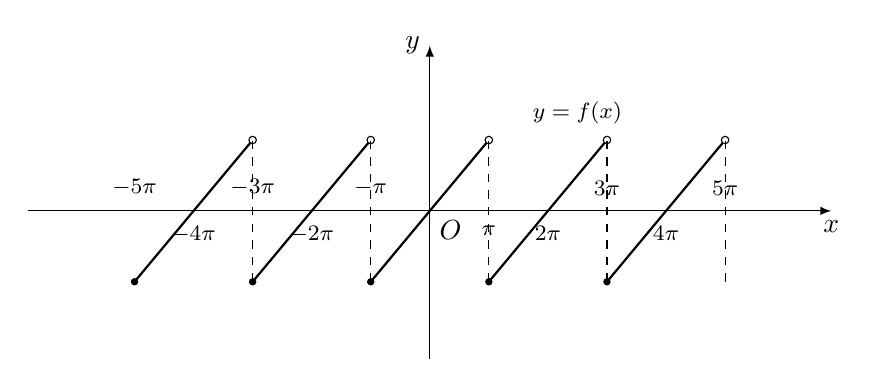
\begin{tikzpicture}[>=latex, scale=0.75]
  \draw[->] (-6.8, 0) -- (6.8, 0) node[below] {$x$};
  \draw[->] (0, -2.5) -- (0, 2.8) node[left] {$y$};
  \node[below right] at (0, 0) {$O$};
  
  \foreach \k in {-2, -1, 0, 1, 2} {
    \draw[thick] (2*\k-1, -1.2) -- (2*\k+1, 1.2);
    \fill (2*\k-1, -1.2) circle (1.8pt);
    \filldraw[fill=white, draw=black] (2*\k+1, 1.2) circle (1.8pt);
    \draw[dashed] (2*\k+1, -1.2) -- (2*\k+1, 1.2);
  }
  
  \draw (-5, 0) node[above=2pt] {\footnotesize $-5\pi$};
  \draw (-4, 0) node[below=2pt] {\footnotesize $-4\pi$};
  \draw (-3, 0) node[above=2pt] {\footnotesize $-3\pi$};
  \draw (-2, 0) node[below=2pt] {\footnotesize $-2\pi$};
  \draw (-1, 0) node[above=2pt] {\footnotesize $-\pi$};
  \draw (1, 0) node[below=2pt] {\footnotesize $\pi$};
  \draw (2, 0) node[below=2pt] {\footnotesize $2\pi$};
  \draw (3, 0) node[above=2pt] {\footnotesize $3\pi$};
  \draw (4, 0) node[below=2pt] {\footnotesize $4\pi$};
  \draw (5, 0) node[above=2pt] {\footnotesize $5\pi$};
  
  \node[above] at (2.5, 1.3) {\footnotesize $y=f(x)$};
\end{tikzpicture}
\caption{}\label{fig:16.1.1}
\end{figure}

\begin{solution}
因为 $x\cos nx$ 与 $x\sin nx$ 分别为奇函数与偶函数, 所以
\[
  a_{n}=\frac{1}{\pi}\int_{-\pi}^{\pi}x\cos nx\,\mathrm{d}x=0,\quad n=0,1,2,\cdots,
\]
\[
  \begin{aligned}
    b_{n}&=\frac{1}{\pi}\int_{-\pi}^{\pi}x\sin nx\,\mathrm{d}x=\frac{2}{\pi}\int_{0}^{\pi}x\sin nx\,\mathrm{d}x=-\frac{2}{n\pi}\int_{0}^{\pi}x\,\mathrm{d}(\cos nx)\\
    &=-\frac{2}{n\pi}\left(\left.x\cos nx\right|_{0}^{\pi}-\int_{0}^{\pi}\cos nx\,\mathrm{d}x\right)=-\frac{2}{n\pi}[\pi(-1)^{n}-0]=(-1)^{n-1}\frac{2}{n},\quad n=1,2,\cdots.
  \end{aligned}
\]
所以,
\[
  f(x)\sim\sum_{n=1}^{\infty}(-1)^{n-1}\frac{2}{n}\sin nx.
\]
根据推论~\ref{cor:16.1.2}, 有
\[
  x=f(x)=\sum_{n=1}^{\infty}(-1)^{n-1}\frac{2}{n}\sin nx,\quad x\in(-\pi,\pi).
\]
进而, 有 (图~\ref{fig:16.1.2})
\[
  \begin{aligned}
    \tilde{f}(x)&=\begin{cases}
      f(x), & x\neq 2k\pi+\pi,\\
      \displaystyle\frac{f(\pi+0)+f(\pi-0)}{2}, & x=2k\pi+\pi,
\end{cases}\quad k=0,\pm 1,\pm 2,\cdots\\
    &=\begin{cases}
      f(x), & x\neq 2k\pi+\pi,\\
      \displaystyle\frac{-\pi+\pi}{2}, & x=2k\pi+\pi,
\end{cases}\quad k=0,\pm 1,\pm 2,\cdots\\
    &=\begin{cases}
      f(x), & x\neq 2k\pi+\pi,\\
      0, & x=2k\pi+\pi,
\end{cases}\quad k=0,\pm 1,\pm 2,\cdots\\
    &=\sum_{n=1}^{\infty}(-1)^{n-1}\frac{2}{n}\sin nx,\quad x\in(-\infty,+\infty).
  \end{aligned}
\]

\begin{figure}[htbp]
\centering
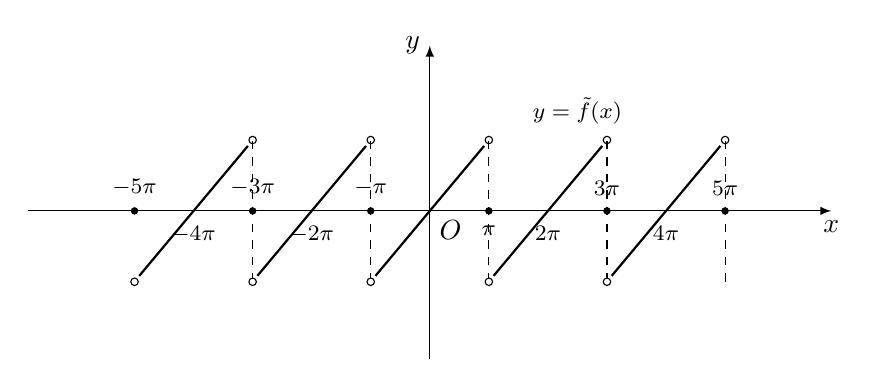
\begin{tikzpicture}[>=latex, scale=0.75]
  \draw[->] (-6.8, 0) -- (6.8, 0) node[below] {$x$};
  \draw[->] (0, -2.5) -- (0, 2.8) node[left] {$y$};
  \node[below right] at (0, 0) {$O$};
  
  \foreach \k in {-2, -1, 0, 1, 2} {
    \draw[thick] (2*\k-0.92, -1.1) -- (2*\k+0.92, 1.1);
    \filldraw[fill=white, draw=black] (2*\k-1, -1.2) circle (1.8pt);
    \filldraw[fill=white, draw=black] (2*\k+1, 1.2) circle (1.8pt);
    \fill (2*\k+1, 0) circle (1.8pt);
    \draw[dashed] (2*\k+1, -1.2) -- (2*\k+1, 1.2);
  }
  \fill (-5, 0) circle (1.8pt);
  
  \draw (-5, 0) node[above=2pt] {\footnotesize $-5\pi$};
  \draw (-4, 0) node[below=2pt] {\footnotesize $-4\pi$};
  \draw (-3, 0) node[above=2pt] {\footnotesize $-3\pi$};
  \draw (-2, 0) node[below=2pt] {\footnotesize $-2\pi$};
  \draw (-1, 0) node[above=2pt] {\footnotesize $-\pi$};
  \draw (1, 0) node[below=2pt] {\footnotesize $\pi$};
  \draw (2, 0) node[below=2pt] {\footnotesize $2\pi$};
  \draw (3, 0) node[above=2pt] {\footnotesize $3\pi$};
  \draw (4, 0) node[below=2pt] {\footnotesize $4\pi$};
  \draw (5, 0) node[above=2pt] {\footnotesize $5\pi$};
  
  \node[above] at (2.5, 1.3) {\footnotesize $y=\tilde{f}(x)$};
\end{tikzpicture}
\caption{}\label{fig:16.1.2}
\end{figure}

取 $x=\displaystyle\frac{\pi}{2}$ 就得到
\[
  \frac{\pi}{2}=\sum_{n=1}^{\infty}(-1)^{n-1}\frac{2}{n}\sin\frac{n\pi}{2},
\]
\[
  \begin{aligned}
    \frac{\pi}{4}&=\sum_{n=1}^{\infty}(-1)^{n-1}\frac{\sin\frac{n\pi}{2}}{n}=\sum_{k=1}^{\infty}(-1)^{2k-2}\frac{\sin\frac{2k-1\pi}{2}}{2k-1}\\
    &=\sum_{k=1}^{\infty}\frac{(-1)^{k-1}}{2k-1}=1-\frac{1}{3}+\frac{1}{5}-\frac{1}{7}+\cdots.
  \end{aligned}
\]
\end{solution}

\begin{example}\label{ex:16.1.2}
设 $f(x)$ 是周期为 $2\pi$ 的函数, 且
\[
  f(x)=\begin{cases}
    x, & x\in(0,2\pi],\\
    2\pi, & x=0.
\end{cases}
\]
求 $f(x)$ 的 Fourier 级数 (图~\ref{fig:16.1.3}) 及函数项级数 $\displaystyle\sum_{n=1}^{\infty}\frac{\sin 2nx}{2n}$, $\displaystyle\sum_{n=1}^{\infty}\frac{\sin 2(n-1)x}{2n-1}$.
\end{example}

\begin{figure}[htbp]
\centering
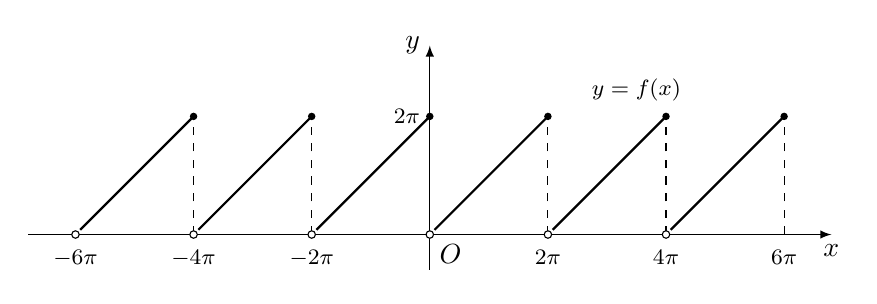
\begin{tikzpicture}[>=latex, scale=0.75]
  \draw[->] (-6.8, 0) -- (6.8, 0) node[below] {$x$};
  \draw[->] (0, -0.6) -- (0, 3.2) node[left] {$y$};
  \node[below right] at (0, 0) {$O$};
  \draw (0, 2) node[left] {\footnotesize $2\pi$};
  
  \foreach \k in {-3, -2, -1, 0, 1, 2} {
    \draw[thick] (2*\k+0.08, 0.08) -- (2*\k+2, 2);
    \filldraw[fill=white, draw=black] (2*\k, 0) circle (1.8pt);
    \fill (2*\k+2, 2) circle (1.8pt);
    \draw[dashed] (2*\k+2, 0) -- (2*\k+2, 2);
  }
  
  \draw (-6, 0) node[below=2pt] {\footnotesize $-6\pi$};
  \draw (-4, 0) node[below=2pt] {\footnotesize $-4\pi$};
  \draw (-2, 0) node[below=2pt] {\footnotesize $-2\pi$};
  \draw (2, 0) node[below=2pt] {\footnotesize $2\pi$};
  \draw (4, 0) node[below=2pt] {\footnotesize $4\pi$};
  \draw (6, 0) node[below=2pt] {\footnotesize $6\pi$};
  
  \node[above] at (3.5, 2.1) {\footnotesize $y=f(x)$};
\end{tikzpicture}
\caption{}\label{fig:16.1.3}
\end{figure}

\begin{solution}
因为
\[
  a_{0}=\frac{1}{\pi}\int_{-\pi}^{\pi}f(x)\,\mathrm{d}x=\frac{1}{\pi}\int_{0}^{2\pi}f(x)\,\mathrm{d}x=\frac{1}{\pi}\int_{0}^{2\pi}x\,\mathrm{d}x=\left.\frac{1}{\pi}\frac{x^{2}}{2}\right|_{0}^{2\pi}=2\pi,
\]
\[
  \begin{aligned}
    a_{n}&=\frac{1}{\pi}\int_{-\pi}^{\pi}f(x)\cos nx\,\mathrm{d}x=\frac{1}{\pi}\int_{0}^{2\pi}f(x)\cos nx\,\mathrm{d}x=\frac{1}{\pi}\int_{0}^{2\pi}x\cos nx\,\mathrm{d}x\\
    &=\frac{1}{n\pi}\int_{0}^{2\pi}x\,\mathrm{d}\sin nx=\frac{1}{n\pi}\left(\left.x\sin nx\right|_{0}^{2\pi}-\int_{0}^{2\pi}\sin nx\,\mathrm{d}x\right)=0,\quad n=1,2,\cdots,
  \end{aligned}
\]
\[
  \begin{aligned}
    b_{n}&=\frac{1}{\pi}\int_{-\pi}^{\pi}f(x)\sin nx\,\mathrm{d}x=\frac{1}{\pi}\int_{0}^{2\pi}f(x)\sin nx\,\mathrm{d}x=\frac{1}{\pi}\int_{0}^{2\pi}x\,\mathrm{d}\left[\frac{\cos nx}{-n}\right]\\
    &=-\frac{1}{n\pi}\left(\left.x\cos nx\right|_{0}^{2\pi}-\int_{0}^{2\pi}\cos nx\,\mathrm{d}x\right)=-\frac{1}{n\pi}(2\pi-0)=-\frac{2}{n},\quad n=1,2,\cdots,
  \end{aligned}
\]
所以,
\[
  f(x)\sim\pi-\sum_{n=1}^{\infty}\frac{2}{n}\sin nx.
\]
根据推论~\ref{cor:16.1.2}, 有
\[
  x=f(x)=\pi-\sum_{n=1}^{\infty}\frac{2}{n}\sin nx,\quad x\in(0,2\pi),
\]
或者
\[
  \frac{\pi-x}{2}=\sum_{n=1}^{\infty}\frac{\sin nx}{n},\quad x\in(0,2\pi).
\]
这正是当年 Abel 给出的例子, 用以说明连续函数项级数的和可能不连续, 根据推论~\ref{cor:13.2.1p}, $\displaystyle\sum_{n=1}^{\infty}\frac{\sin nx}{n}$ 在 $[0,2\pi]$ 上不一致收敛.

进而, 有 (图~\ref{fig:16.1.4})
\[
  \begin{aligned}
    \tilde{f}(x)&=\begin{cases}
      f(x), & x\neq 2k\pi,\\
      \displaystyle\frac{f(0+0)+f(0-0)}{2}, & x=2k\pi,
\end{cases}\quad k=0,\pm 1,\pm 2,\cdots\\
    &=\begin{cases}
      f(x), & x\neq 2k\pi,\\
      \displaystyle\frac{0+2\pi}{2}, & x=2k\pi,
\end{cases}\quad k=0,\pm 1,\pm 2,\cdots\\
    &=\begin{cases}
      f(x), & x\neq 2k\pi,\\
      \pi, & x=2k\pi,
\end{cases}\quad k=0,\pm 1,\pm 2,\cdots\\
    &=\pi-\sum_{n=1}^{\infty}\frac{2}{n}\sin nx,\quad x\in(-\infty,+\infty).
  \end{aligned}
\]

\begin{figure}[htbp]
\centering
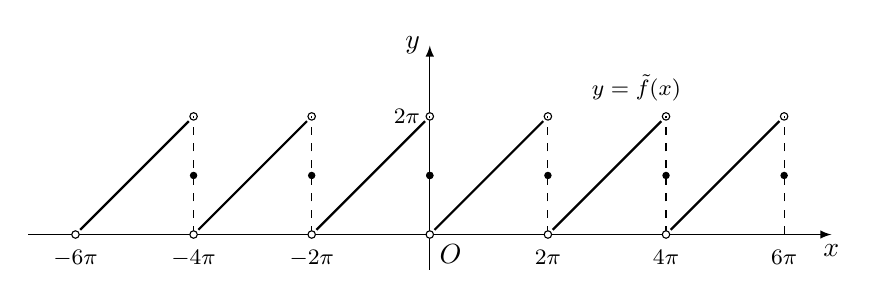
\begin{tikzpicture}[>=latex, scale=0.75]
  \draw[->] (-6.8, 0) -- (6.8, 0) node[below] {$x$};
  \draw[->] (0, -0.6) -- (0, 3.2) node[left] {$y$};
  \node[below right] at (0, 0) {$O$};
  \draw (0, 2) node[left] {\footnotesize $2\pi$};
  
  \foreach \k in {-3, -2, -1, 0, 1, 2} {
    \draw[thick] (2*\k+0.08, 0.08) -- (2*\k+1.92, 1.92);
    \filldraw[fill=white, draw=black] (2*\k, 0) circle (1.8pt);
    \filldraw[fill=white, draw=black] (2*\k+2, 2) circle (1.8pt);
    \fill (2*\k+2, 1) circle (1.8pt);
    \draw[dashed] (2*\k+2, 0) -- (2*\k+2, 2);
  }
  \fill (0, 1) circle (1.8pt);
  
  \draw (-6, 0) node[below=2pt] {\footnotesize $-6\pi$};
  \draw (-4, 0) node[below=2pt] {\footnotesize $-4\pi$};
  \draw (-2, 0) node[below=2pt] {\footnotesize $-2\pi$};
  \draw (2, 0) node[below=2pt] {\footnotesize $2\pi$};
  \draw (4, 0) node[below=2pt] {\footnotesize $4\pi$};
  \draw (6, 0) node[below=2pt] {\footnotesize $6\pi$};
  
  \node[above] at (3.5, 2.1) {\footnotesize $y=\tilde{f}(x)$};
\end{tikzpicture}
\caption{}\label{fig:16.1.4}
\end{figure}

从
\[
  \frac{\pi-x}{2}=\sum_{n=1}^{\infty}\frac{\sin nx}{n},\quad x\in(0,2\pi)
\]
不经计算可得到其他一些有趣的等式. 例如, 将 $x$ 换成 $2x$ 便可得到
\[
  \frac{\pi}{4}-\frac{x}{2}=\sum_{n=1}^{\infty}\frac{\sin 2nx}{2n},\quad x\in(0,\pi).
\]
两式相减就有
\[
  \frac{\pi}{4}=\sum_{n=1}^{\infty}\frac{\sin(2n-1)x}{2n-1},\quad x\in(0,\pi).
\]
令 $x=\displaystyle\frac{\pi}{2}$, 再一次得到
\[
  \frac{\pi}{4}=\sum_{n=1}^{\infty}\frac{\sin(2n-1)\frac{\pi}{2}}{2n-1}=\sum_{n=1}^{\infty}\frac{(-1)^{n-1}}{2n-1}=1-\frac{1}{3}+\frac{1}{5}-\frac{1}{7}+\cdots.
\]
\end{solution}
\begin{example}\label{ex:16.1.3}
将函数 $f(x)=x^{2}$, $x\in[-\pi,\pi]$ 展开为 Fourier 级数. 由此证明:
\[
  \sum_{n=1}^{\infty}\frac{1}{x^{2}}=\frac{\pi^{2}}{6},\quad\sum_{n=1}^{\infty}\frac{(-1)^{n-1}}{n^{2}}=\frac{\pi^{2}}{12}.% 原书如此: 印刷为 x^2, 实为 n^2
\]
\end{example}

\begin{solution}
将 $f(x)$ 的定义延拓到整个数轴上, 使之成为周期为 $2\pi$ 的函数 (图~\ref{fig:16.1.5}), 记延拓后的函数为 $\tilde{f}(x)$, 则 $\tilde{f}(x)$ 是 $(-\infty,+\infty)$ 上的周期为 $2\pi$ 的连续偶函数. 于是,
\[
  a_{0}=\frac{1}{\pi}\int_{-\pi}^{\pi}f(x)\,\mathrm{d}x=\frac{2}{\pi}\int_{0}^{\pi}x^{2}\,\mathrm{d}x=\left.\frac{2}{\pi}\frac{x^{3}}{3}\right|_{0}^{\pi}=\frac{2}{3}\pi^{2},
\]
\[
  \begin{aligned}
    a_{n}&=\frac{1}{\pi}\int_{-\pi}^{\pi}f(x)\cos nx\,\mathrm{d}x=\frac{2}{\pi}\int_{0}^{\pi}x^{2}\cos nx\,\mathrm{d}x=\frac{2}{n\pi}\int_{0}^{\pi}x^{2}\,\mathrm{d}\sin nx\\
    &=\frac{2}{n\pi}\left(\left.x^{2}\sin nx\right|_{0}^{\pi}-\int_{0}^{\pi}2x\sin nx\,\mathrm{d}x\right)=\frac{4}{n^{2}\pi}\int_{0}^{\pi}x\,\mathrm{d}\cos nx\\
    &=\frac{4}{n^{2}\pi}\left(\left.x\cos nx\right|_{0}^{\pi}-\int_{0}^{\pi}cos nx\,\mathrm{d}x\right)=\frac{4}{n^{2}\pi}[\pi(-1)^{n}-0]=(-1)^{n}\frac{4}{n^{2}},\quad n=1,2,\cdots,
  \end{aligned}
\]
\[
  b_{n}=\frac{1}{\pi}\int_{-\pi}^{\pi}f(x)\sin nx\,\mathrm{d}x=\frac{1}{\pi}\int_{-\pi}^{\pi}x^{2}\sin nx\,\mathrm{d}x\xlongequal{\text{奇函数}}0,\quad n=1,2,\cdots.
\]

\begin{figure}[htbp]
\centering
\begin{tikzpicture}[>=latex, scale=0.8]
  \draw[->] (-10.5, 0) -- (10.5, 0) node[below] {$x$};
  \draw[->] (0, -0.6) -- (0, 3.8) node[left] {$y$};
  \node[below right] at (0, 0) {$O$};
  \draw (0, 3.1) node[left] {\footnotesize $\pi^2$};
  
  \foreach \k in {-1, 0, 1} {
    \draw[thick, smooth, domain=-3.14159:3.14159, variable=\t] plot ({2*\k*3.14159/1.8 + \t/1.8}, {(\t)^2 / (3.14159^2) * 3.1});
  }
  
  \draw (-3*3.14159/1.8, 0) node[below=2pt] {\footnotesize $-3\pi$};
  \draw (-2*3.14159/1.8, 0) node[below=2pt] {\footnotesize $-2\pi$};
  \draw (-3.14159/1.8, 0) node[below=2pt] {\footnotesize $-\pi$};
  \draw (3.14159/1.8, 0) node[below=2pt] {\footnotesize $\pi$};
  \draw (2*3.14159/1.8, 0) node[below=2pt] {\footnotesize $2\pi$};
  \draw (3*3.14159/1.8, 0) node[below=2pt] {\footnotesize $3\pi$};
  
  \draw[dashed] (-3*3.14159/1.8, 0) -- (-3*3.14159/1.8, 3.1);
  \draw[dashed] (3*3.14159/1.8, 0) -- (3*3.14159/1.8, 3.1);
  
  \node[above] at (1.8*3.14159/1.8, 3.1) {\footnotesize $y=\tilde{f}(x)$};
\end{tikzpicture}
\caption{}\label{fig:16.1.5}
\end{figure}

根据推论~\ref{cor:16.1.2}, 有
\[
  \tilde{f}(x)=\frac{\pi^{2}}{3}+4\sum_{n=1}^{\infty}\frac{(-1)^{n}}{n^{2}}\cos nx,\quad x\in(-\infty,+\infty).
\]
限制在区间 $[-\pi,\pi]$ 上有
\[
  x^{2}=f(x)=\frac{\pi^{2}}{3}+4\sum_{n=1}^{\infty}\frac{(-1)^{n}}{n^{2}}\cos nx,\quad x\in[-\pi,\pi],
\]
或者
\[
  \sum_{n=1}^{\infty}(-1)^{n}\frac{\cos nx}{n^{2}}=\frac{x^{2}}{4}-\frac{\pi^{2}}{12},\quad x\in[-\pi,\pi].
\]
令 $x=\pi$ 就得
\[
  \sum_{n=1}^{\infty}\frac{1}{n^{2}}=\frac{\pi^{2}}{4}-\frac{\pi^{2}}{12}=\frac{\pi^{2}}{6}.
\]
令 $x=0$ 就得
\[
  \sum_{n=1}^{\infty}\frac{(-1)^{n}}{n^{2}}=\frac{0^{2}}{4}-\frac{\pi^{2}}{12}=-\frac{\pi^{2}}{12},
\]
\[
  \sum_{n=1}^{\infty}\frac{(-1)^{n-1}}{n^{2}}=\frac{\pi^{2}}{12}.
\]
\end{solution}

\begin{example}\label{ex:16.1.4}
设 $a$ 不为整数, 将 $f(x)=\cos ax$ 在 $[-\pi,\pi]$ 上展开为 Fourier 级数并证明
\[
  \frac{\pi}{\sin a\pi}=\frac{1}{a}+\sum_{n=1}^{\infty}(-1)^{n}\frac{2a}{a^{2}-n^{2}},\quad a\notin\mathbb{Z}.
\]
\end{example}

\begin{solution}
将 $f(x)$ 延拓为整个数轴上的以 $2\pi$ 为周期的函数, 记延拓后的函数为 $\tilde{f}(x)$, 则 $\tilde{f}(x)$ 是 $(-\infty,+\infty)$ 上的周期为 $2\pi$ 的连续偶函数. 因此,
\[
  a_{n}=\frac{1}{n}\int_{-\pi}^{\pi}f(x)\cos ax\,\mathrm{d}x=\frac{2}{\pi}\int_{0}^{\pi}\cos ax\cos nx\,\mathrm{d}x% 原书如此: 印刷为 \frac{1}{n} 和 \cos ax
\]
\[
  \begin{aligned}
    &=\frac{1}{\pi}\int_{0}^{\pi}[\cos(a-n)x+\cos(a+n)x]\,\mathrm{d}x=\left.\frac{1}{\pi}\left[\frac{\sin(a-n)x}{a-n}+\frac{\sin(a+n)x}{a+n}\right]\right|_{0}^{\pi}\\
    &=\frac{1}{\pi}\left[\frac{\sin(a-n)\pi}{a-n}+\frac{\sin(a+n)\pi}{a+n}\right]=\frac{1}{\pi}\left[\frac{(-1)^{n}\sin a\pi}{a-n}+\frac{(-1)^{n}\sin a\pi}{a+n}\right]\\
    &=\frac{(-1)^{n}}{\pi}\frac{2a\sin a\pi}{a^{2}-n^{2}},\quad n=0,1,2,\cdots,
  \end{aligned}
\]
\[
  b_{n}=\frac{1}{\pi}\int_{-\pi}^{\pi}f(x)\sin ax\,\mathrm{d}x=\frac{1}{\pi}\int_{-\pi}^{\pi}\cos ax\sin nx\,\mathrm{d}x\xlongequal{\text{奇函数}}0,\quad n=1,2,\cdots.% 原书如此: 前式印刷为 \sin ax
\]
根据推论~\ref{cor:16.1.2}, 可知 $\tilde{f}(x)$ 的 Fourier 级数为
\[
  \tilde{f}(x)=\frac{\sin a\pi}{\pi}\left[\frac{1}{a}+\sum_{n=1}^{\infty}(-1)^{n}\frac{2a}{a^{2}-n^{2}}\cos nx\right],\quad x\in(-\infty,+\infty).
\]
限制在 $[-\pi,\pi]$ 上就有
\[
  \cos ax=\frac{\sin a\pi}{\pi}\left[\frac{1}{a}+\sum_{n=1}^{\infty}(-1)^{n}\frac{2a}{a^{2}-n^{2}}\cos nx\right],\quad x\in[-\pi,\pi].
\]
如果在上式中, 令 $x=0$, 就可得
\[
  \frac{\pi}{\sin a\pi}=\frac{1}{a}+\sum_{n=1}^{\infty}(-1)^{n}\frac{2a}{a^{2}-n^{2}},\quad a\notin\mathbb{Z}.
\]
\end{solution}

应用例~\ref{ex:16.1.4} 中的公式
\[
  \frac{\pi}{\sin a\pi}=\frac{1}{a}+\sum_{n=1}^{\infty}(-1)^{n}\frac{2a}{a^{2}-n^{2}},\quad a\notin\mathbb{Z}
\]
可以计算出下面积分的值.

\begin{example}\label{ex:16.1.5}
证明: 无穷积分
\[
  \int_{0}^{+\infty}\frac{x^{p-1}}{1+x}\,\mathrm{d}x=\frac{1}{p}+\sum_{n=1}^{\infty}(-1)^{n}\frac{2p}{p^{2}-n^{2}}=\frac{\pi}{\sin p\pi},\quad 0<p<1.
\]
\end{example}

\begin{proof}
当 $0<x<1$ 时, 有展开式
\[
  \frac{x^{p-1}}{1+x}=\sum_{n=0}^{\infty}(-1)^{n}x^{n+p-1},
\]
且这个级数在区间 $(0,1)$ 的任何内闭区间 $[a,b]\subset(0,1)$ 上都一致收敛, 如果记它的部分和为 $f_{n}(x)$, 则 $\{f_{n}(x)\}$ 在区间 $(0,1)$ 的任何内闭区间 $[a,b]\subset(0,1)$ 上一致收敛. 由于
\[
  0\leqslant f_{n}(x)=\sum_{k=0}^{n-1}(-1)^{k}x^{k+p-1}=\frac{x^{p-1}[1-(-1)^{n}x^{n}]}{1+x}\leqslant 2\cdot\frac{x^{p-1}}{1+x}\leqslant 2x^{p-1},
\]
而 $\displaystyle\int_{0}^{1}x^{p-1}\,\mathrm{d}x$ 收敛, 故 $\displaystyle\int_{0}^{1}f_{n}(x)\,\mathrm{d}x$ 关于 $n$ 一致收敛.
\[
  \begin{aligned}
    \int_{0}^{1}\frac{x^{p-1}}{1+x}\,\mathrm{d}x&=\int_{0}^{1}\sum_{n=0}^{\infty}(-1)^{n}x^{n+p-1}\,\mathrm{d}x\xlongequal{\text{定理~\ref{thm:15.2.6}}}\sum_{n=0}^{\infty}(-1)^{n}\int_{0}^{1}x^{n+p-1}\,\mathrm{d}x\\
    &=\sum_{n=0}^{\infty}\frac{(-1)^{n}}{n+p}.
  \end{aligned}
\]
进而, 有
\[
  \begin{aligned}
    \int_{1}^{+\infty}\frac{x^{p-1}}{1+x}\,\mathrm{d}x&\xlongequal{x=\frac{1}{t}}\int_{1}^{0}\frac{\left(\frac{1}{t}\right)^{p-1}}{1+\frac{1}{t}}\cdot\frac{-1}{t^{2}}\,\mathrm{d}t=\int_{0}^{1}\frac{t^{-p}}{1+t}\,\mathrm{d}t\\
    &=\int_{0}^{1}\frac{t^{(1-p)+1}}{1+t}\,\mathrm{d}t\xlongequal{\text{由上面结果}}\sum_{n=0}^{\infty}\frac{(-1)^{n}}{n+1-p}=\sum_{n=1}^{\infty}\frac{(-1)^{n}}{p-n}.% 原书如此: 印刷为 t^{(1-p)+1}
  \end{aligned}
\]
综合上述得到
\[
  \begin{aligned}
    \int_{0}^{+\infty}\frac{x^{p-1}}{1+x}\,\mathrm{d}x&=\int_{0}^{1}\frac{x^{p-1}}{1+x}\,\mathrm{d}x+\int_{1}^{+\infty}\frac{x^{p-1}}{1+x}\,\mathrm{d}x\\
    &=\sum_{n=0}^{\infty}\frac{(-1)^{n}}{p+n}+\sum_{n=1}^{\infty}\frac{(-1)^{n}}{p-n}=\frac{1}{p}+\sum_{n=1}^{\infty}(-1)^{n}\frac{2p}{p^{2}-n^{2}}\\
    &\xlongequal{\text{例~\ref{ex:16.1.4}}}\frac{\pi}{\sin p\pi},\quad 0<p<1.
  \end{aligned}
\]
\end{proof}

\begin{example}\label{ex:16.1.6}
将函数 $\mathrm{e}^{ax}$ 在区间 $(0,2\pi)$ 上展开为 Fourier 级数, 并求 $\displaystyle\sum_{n=1}^{\infty}\frac{1}{1+n^{2}}$.
\end{example}

\begin{solution}
先计算 Fourier 系数:
\[
  \begin{aligned}
    a_{n}&=\frac{1}{\pi}\int_{0}^{2\pi}\mathrm{e}^{ax}\cos nx\,\mathrm{d}x=\left.\frac{1}{\pi}\frac{\mathrm{e}^{ax}}{a^{2}+n^{2}}(a\cos nx+n\sin nx)\right|_{0}^{2\pi}\\
    &=\frac{\mathrm{e}^{2\pi a}-1}{\pi}\frac{a}{a^{2}+n^{2}},\quad n=0,1,2,\cdots.
  \end{aligned}
\]
\[
  \begin{aligned}
    b_{n}&=\frac{1}{\pi}\int_{0}^{2\pi}\mathrm{e}^{ax}\sin nx\,\mathrm{d}x=\left.\frac{1}{\pi}\frac{\mathrm{e}^{ax}}{a^{2}+n^{2}}(a\sin nx-n\cos nx)\right|_{0}^{2\pi}\\
    &=\frac{\mathrm{e}^{2\pi a}-1}{\pi}\frac{-n}{a^{2}+n^{2}},\quad n=1,2,\cdots.
  \end{aligned}
\]
于是,
\[
  \mathrm{e}^{ax}=\frac{\mathrm{e}^{2\pi a}-1}{\pi}\left(\frac{1}{2a}+\sum_{n=1}^{\infty}\frac{a\cos nx-n\sin nx}{a^{2}+n^{2}}\right),\quad 0<x<2\pi.
\]
如果将 $f(x)=\mathrm{e}^{ax}$ ($0<x<2\pi$) 延拓为 $(-\infty,+\infty)$ 上以 $2\pi$ 为周期的函数 $\tilde{f}(x)$, 则必须有
\[
  \tilde{f}(0)=\tilde{f}(2\pi)=\frac{f(2\pi-0)+f(0+0)}{2}=\frac{\mathrm{e}^{2\pi a}+\mathrm{e}^{0\cdot a}}{2}=\frac{\mathrm{e}^{2\pi a}+1}{2}.
\]
由此得到
\[
  \tilde{f}(x)=\frac{\mathrm{e}^{2\pi a}-1}{\pi}\left(\frac{1}{2a}+\sum_{n=1}^{\infty}\frac{a\cos nx-n\sin nx}{a^{2}+n^{2}}\right),\quad -\infty<x<+\infty.
\]
令 $a=1$, $x=0$, 就有
\[
  \frac{\mathrm{e}^{2\pi}+1}{2}=\frac{\mathrm{e}^{2\pi}-1}{\pi}\left(\frac{1}{2}+\sum_{n=1}^{\infty}\frac{1}{1+n^{2}}\right),
\]
即
\[
  \sum_{n=1}^{\infty}\frac{1}{1+n^{2}}=\frac{\mathrm{e}^{2\pi}+1}{2}\cdot\frac{\pi}{\mathrm{e}^{2\pi}-1}-\frac{1}{2}=\frac{\pi}{2}\frac{\mathrm{e}^{2\pi}+1}{\mathrm{e}^{2\pi}-1}-\frac{1}{2}.
\]
\end{solution}

\begin{remark}\label{rem:16.1.2}
从例~\ref{ex:16.1.1}$\sim$例~\ref{ex:16.1.4}, 例~\ref{ex:16.1.6} 可看到, 经某个函数的 Fourier 级数的计算, 并取特殊点求得一些数项级数之和, 这些数项级数之和是难以用其他方法得到的.
\end{remark}

上面各例都是先给出函数在 $(-\pi,\pi)$ 或 $(0,2\pi)$ 上的表达式, 然后将它延拓为整个数轴上的周期 $2\pi$ 的函数, 再将它展开为 Fourier 级数.

对于只在 $(0,\pi)$ 上定义的函数, 如何展开为 Fourier 级数呢? 这时, 在 $(-\pi,0)$ 上可以任意补充 $f(x)$ 的定义, 使 $f(x)$ 在 $(-\pi,\pi)$ 上有定义, 然后再将它以 $2\pi$ 为周期延拓到整个数轴上去. 对于各种不同的延拓, 得到的 Fourier 级数自然也是不同的. 但在 $(0,\pi)$ 上, 它们都收敛到同一个函数. 而偶性延拓与奇性延拓是常用的两种延拓方法.

\begin{definition}\label{def:16.1.3}
设 $f(x)$ 是定义在 $(0,\pi)$ 上的函数, 令
\[
  f(x)=f(-x),\quad x\in(-\pi,0)
\]
来补充 $f(x)$ 在 $(-\pi,0)$ 上的定义, 使 $f(x)$ 在 $(-\pi,\pi)$ 上成为偶函数 (延拓后的函数 $\tilde{f}(x)$ 仍记为 $f(x)$), 这种延拓方法称为\textbf{偶性延拓}. 这样便有
\[
  a_{n}=\frac{1}{\pi}\int_{-\pi}^{\pi}f(x)\cos nx\,\mathrm{d}x=\frac{2}{\pi}\int_{0}^{\pi}f(x)\cos nx\,\mathrm{d}x,\quad n=0,1,2,\cdots,
\]
\[
  b_{n}=\frac{1}{\pi}\int_{-\pi}^{\pi}f(x)\sin nx\,\mathrm{d}x=0,\quad n=1,2,\cdots.
\]
因此, $f(x)$ 的 Fourier 级数中只含余弦项:
\[
  f(x)\sim\frac{a_{0}}{2}+\sum_{n=1}^{\infty}a_{n}\cos nx,
\]
称它为 $f(x)$, $x\in(0,\pi)$ 的\textbf{余弦级数}.

如果令
\[
  f(x)=-f(-x),\quad x\in(-\pi,0)
\]
来补充 $f(x)$ 在 $(-\pi,0)$ 上的定义, 使 $f(x)$ 在 $(-\pi,\pi)$ 上成为奇函数 (延拓后的函数 $\tilde{f}(x)$ 仍记为 $f(x)$), 这种延拓方法称为\textbf{奇性延拓} (注意: 由 $f(0)=f(-0)=-f(0)$, 知 $f(0)=0$). 这样便有
\[
  a_{n}=\frac{1}{\pi}\int_{-\pi}^{\pi}f(x)\cos nx\,\mathrm{d}x=0,\quad n=0,1,2,\cdots,
\]
\[
  b_{n}=\frac{1}{\pi}\int_{-\pi}^{\pi}f(x)\sin nx\,\mathrm{d}x=\frac{2}{\pi}\int_{0}^{\pi}f(x)\sin nx\,\mathrm{d}x,\quad n=1,2,\cdots.
\]
因此, $f(x)$ 的 Fourier 级数中只含正弦项:
\[
  f(x)\sim\sum_{n=1}^{\infty}b_{n}\sin nx,
\]
称它为 $f(x)$, $x\in(0,\pi)$ 的\textbf{正弦级数}.
\end{definition}

由此可见, 对于只定义在区间 $(0,\pi)$ 上的函数, 只要满足 Dini 定理的条件, 就可考虑它的正弦级数, 也可考虑它的余弦级数.

\begin{example}\label{ex:16.1.7}
将函数
\[
  f(x)=x,\quad x\in(0,\pi)
\]
分别展开为余弦级数与正弦级数.
\end{example}

\begin{solution}
若要展开成余弦级数, 可先将 $f(x)$, $x\in(0,\pi)$ 偶性延拓到区间 $(-\pi,0)$ 上, 然后再将它以周期 $2\pi$ 延拓到整个区间 $(-\infty,+\infty)$ 上, 所得的函数记为 $\tilde{f}(x)$ (图~\ref{fig:16.1.6}). 于是,
\[
  a_{0}=\frac{2}{\pi}\int_{0}^{\pi}x\,\mathrm{d}x=\pi,
\]
\[
  \begin{aligned}
    a_{n}&=\frac{2}{\pi}\int_{0}^{\pi}x\cos nx\,\mathrm{d}x=\frac{2}{n\pi}\int_{0}^{\pi}x\,\mathrm{d}\sin nx\\
    &=\frac{2}{n\pi}\left(\left.x\sin nx\right|_{0}^{\pi}-\int_{0}^{\pi}\sin nx\,\mathrm{d}x\right)=\left.\frac{2}{n^{2}\pi}\cos nx\right|_{0}^{\pi}\\
    &=\frac{2}{n^{2}\pi}[(-1)^{n}-1]=\begin{cases}
      0, & n=2k,\\
      \displaystyle-\frac{4}{(2k-1)^{2}\pi}, & n=2k-1,
\end{cases}\quad k=1,2,\cdots,
  \end{aligned}
\]
\[
  b_{n}=0,\quad n=1,2,\cdots.
\]
所以,
\[
  x=\frac{\pi}{2}-\frac{4}{\pi}\sum_{k=1}^{\infty}\frac{\cos(2k-1)x}{(2k-1)^{2}},\quad x\in[0,\pi].% 原书如此: 公式中分子印刷为 \cos(2k-1)\pi
\]
\[
  \tilde{f}(x)=\frac{\pi}{2}-\frac{4}{\pi}\sum_{k=1}^{\infty}\frac{\cos(2k-1)x}{(2k-1)^{2}},\quad x\in(-\infty,+\infty).% 原书如此: 同样印刷为 \cos(2k-1)\pi
\]

\begin{figure}[htbp]
\centering
\begin{tikzpicture}[>=latex, scale=0.85]
  \draw[->] (-7.5, 0) -- (7.5, 0) node[below] {$x$};
  \draw[->] (0, -0.6) -- (0, 3.2) node[left] {$y$};
  \node[below right] at (0, 0) {$O$};
  
  % 刻度标记
  \draw (-2*2.2, 0) node[below=2pt] {\footnotesize $-2\pi$};
  \draw (-2.2, 0) node[below=2pt] {\footnotesize $-\pi$};
  \draw (2.2, 0) node[below=2pt] {\footnotesize $\pi$};
  \draw (2*2.2, 0) node[below=2pt] {\footnotesize $2\pi$};
  
  % 折线段
  \draw[thick] (-2*2.2, 0) -- (-2.2, 2.2);
  \draw[thick, dashed] (-2.2, 2.2) -- (0, 0);
  \draw[thick] (0, 0) -- (2.2, 2.2) -- (2*2.2, 0);
  \draw[thick] (-2*2.2, 0) -- (-2.6*2.2, 0.6*2.2);
  \draw[thick] (2*2.2, 0) -- (2.6*2.2, 0.6*2.2);
\end{tikzpicture}
\caption{}\label{fig:16.1.6}
\end{figure}

令 $x=0$ 得
\[
  \sum_{k=1}^{\infty}\frac{1}{(2k-1)^{2}}=\frac{\pi^{2}}{8}.
\]
此数项级数之和也可如下得到:
\[
  \sum_{n=1}^{\infty}\frac{1}{n^{2}}=\sum_{k=1}^{\infty}\frac{1}{(2k-1)^{2}}+\sum_{k=1}^{\infty}\frac{1}{(2k)^{2}},
\]
\[
  \sum_{k=1}^{\infty}\frac{1}{(2k-1)^{2}}=\sum_{n=1}^{\infty}\frac{1}{n^{2}}-\sum_{k=1}^{\infty}\frac{1}{(2k)^{2}}=\frac{3}{4}\sum_{n=1}^{\infty}\frac{1}{n^{2}}\xlongequal{\text{例~\ref{ex:16.1.3}}}\frac{3}{4}\times\frac{\pi^{2}}{6}=\frac{\pi^{2}}{8}.
\]
若要展开成正弦级数, 可先将 $f(x)$, $x\in(0,\pi)$ 奇性延拓到 $(-\pi,0)$ 上, 然后再将它以周期 $2\pi$ 延拓到整个区间 $(-\infty,+\infty)$ 上, 所得的函数记为 $\tilde{f}(x)$ (图~\ref{fig:16.1.7}). 于是, 由例~\ref{ex:16.1.1} 知
\[
  x=2\sum_{n=1}^{\infty}(-1)^{n-1}\frac{\sin nx}{n},\quad x\in[0,\pi).
\]

\begin{figure}[htbp]
\centering
\begin{tikzpicture}[>=latex, scale=0.85]
  \draw[->] (-8.5, 0) -- (8.5, 0) node[below] {$x$};
  \draw[->] (0, -2.6) -- (0, 2.8) node[left] {$y$};
  \node[below right] at (0, 0) {$O$};
  
  % 刻度标记
  \draw (-3*2.2, 0) node[below=2pt] {\footnotesize $-3\pi$};
  \draw (-2*2.2, 0) node[below=2pt] {\footnotesize $-2\pi$};
  \draw (-2.2, 0) node[below=2pt] {\footnotesize $-\pi$};
  \draw (2.2, 0) node[below=2pt] {\footnotesize $\pi$};
  \draw (2*2.2, 0) node[below=2pt] {\footnotesize $2\pi$};
  \draw (3*2.2, 0) node[below=2pt] {\footnotesize $3\pi$};
  
  % 中间周期
  \draw[thick, dashed] (-2.2+0.05, -1.8+0.05) -- (0, 0);
  \draw[thick] (0, 0) -- (2.2-0.05, 1.8-0.05);
  \filldraw[fill=white, draw=black] (-2.2, -1.8) circle (1.8pt);
  \filldraw[fill=white, draw=black] (2.2, 1.8) circle (1.8pt);
  
  % 右侧周期
  \draw[thick] (2.2+0.05, -1.8+0.05) -- (3*2.2-0.05, 1.8-0.05);
  \filldraw[fill=white, draw=black] (2.2, -1.8) circle (1.8pt);
  \filldraw[fill=white, draw=black] (3*2.2, 1.8) circle (1.8pt);
  
  % 左侧周期
  \draw[thick] (-3*2.2+0.05, -1.8+0.05) -- (-2.2-0.05, 1.8-0.05);
  \filldraw[fill=white, draw=black] (-3*2.2, -1.8) circle (1.8pt);
  \filldraw[fill=white, draw=black] (-2.2, 1.8) circle (1.8pt);
\end{tikzpicture}
\caption{}\label{fig:16.1.7}
\end{figure}

如果 $\tilde{f}[(2k-1)\pi]=\frac{\pi+(-\pi)}{2}=0$, 则
\[
  \tilde{f}(x)=2\sum_{n=1}^{\infty}(-1)^{n-1}\frac{\sin nx}{n},\quad x\in(-\infty,+\infty).
\]
\end{solution}

下面来讨论周期为 $2l$ 的函数的 Fourier 展开.

\begin{definition}\label{def:16.1.4}
设 $f(x)$ 是以 $2l$ 为周期的函数, 作变换 $x=\frac{l}{\pi}t$, 并记
\[
  f(x)=f\left(\frac{l}{\pi}t\right)=g(t),
\]
则 $g(t)$ 是周期为 $2\pi$ 的函数. 如果 $g(t)$ 满足 Dini 定理推论的条件, 便有
\[
  g(t)=\frac{a_{0}}{2}+\sum_{n=1}^{\infty}(a_{n}\cos nt+b_{n}\sin nt),\quad t\in(-\infty,+\infty),
\]
其中
\[
  a_{n}=\frac{1}{\pi}\int_{-\pi}^{\pi}g(t)\cos nt\,\mathrm{d}t,\quad n=0,1,2,\cdots,
\]
\[
  b_{n}=\frac{1}{\pi}\int_{-\pi}^{\pi}g(t)\sin nt\,\mathrm{d}t,\quad n=1,2,\cdots.
\]
回到原来的变量 $x$ 就有
\[
  f(x)=\frac{a_{0}}{2}+\sum_{n=1}^{\infty}\left(a_{n}\cos\frac{n\pi}{l}x+b_{n}\sin\frac{n\pi}{l}x\right),\quad x\in(-\infty,+\infty),
\]
而
\[
  \begin{aligned}
    a_{n}&=\frac{1}{\pi}\int_{-\pi}^{\pi}g(t)\cos nt\,\mathrm{d}t\xlongequal{t=\frac{\pi}{l}x}\frac{1}{\pi}\int_{-l}^{l}f(x)\cos\frac{n\pi}{l}x\,\mathrm{d}\left(\frac{\pi}{l}x\right)\\
    &=\frac{1}{l}\int_{-l}^{l}f(x)\cos\frac{n\pi}{l}x\,\mathrm{d}x,\quad n=0,1,2,\cdots,
  \end{aligned}
\]
\[
  \begin{aligned}
    b_{n}&=\frac{1}{\pi}\int_{-\pi}^{\pi}g(t)\sin nt\,\mathrm{d}t\xlongequal{t=\frac{\pi}{l}x}\frac{1}{\pi}\int_{-l}^{l}f(x)\sin\frac{n\pi}{l}x\,\mathrm{d}\left(\frac{\pi}{l}x\right)\\
    &= \frac{1}{l}\int_{-l}^{l}f(x)\sin\frac{n\pi}{l}x\,\mathrm{d}x,\quad n=1,2,\cdots.
  \end{aligned}
\]
这就给出了周期 $2l$ 的函数 $f(x)$ 的 Fourier 展开式.

如果 $f(x)$ 只定义在 $(0,l)$ 上, 则它既可展开为余弦级数
\[
  f(x)=\frac{a_{0}}{2}+\sum_{n=1}^{\infty}a_{n}\cos\frac{n\pi}{l}x,
\]
其中
\[
  a_{n}=\frac{2}{l}\int_{0}^{l}f(x)\cos\frac{n\pi}{l}x\,\mathrm{d}x,\quad n=0,1,2,\cdots,
\]
也可展开为正弦级数
\[
  f(x)=\sum_{n=1}^{\infty}b_{n}\sin\frac{n\pi}{l}x,
\]
其中
\[
  b_{n}=\frac{2}{l}\int_{0}^{l}f(x)\sin\frac{n\pi}{l}x\,\mathrm{d}x,\quad n=1,2,\cdots.
\]
\end{definition}

\begin{example}\label{ex:16.1.8}
将函数
\[
  f(x)=\begin{cases}
    x, & x\in\left[0,\dfrac{l}{2}\right],\\
    l-x, & x\in\left[\dfrac{l}{2},l\right]
\end{cases}
\]
在 $[0,l]$ 上展开为正弦级数.
\end{example}

\begin{solution}
将 $f(x)$ 作奇性延拓 (图~\ref{fig:16.1.8}) 得 $\tilde{f}(x)$, 则
\[
  \begin{aligned}
    b_{n}&=\frac{2}{l}\int_{0}^{l}f(x)\sin\frac{n\pi}{l}x\,\mathrm{d}x\\
    &=\frac{2}{l}\int_{0}^{\frac{l}{2}}x\sin\frac{n\pi}{l}x\,\mathrm{d}x+\frac{2}{l}\int_{\frac{l}{2}}^{l}(l-x)\sin\frac{n\pi}{l}x\,\mathrm{d}x\\
    &=\frac{2}{l}\int_{0}^{\frac{l}{2}}x\,\mathrm{d}\left(-\frac{l}{n\pi}\cos\frac{n\pi}{l}x\right)+\frac{2}{l}\int_{\frac{l}{2}}^{l}(l-x)\,\mathrm{d}\left(-\frac{l}{n\pi}\cos\frac{n\pi}{l}x\right)\\
    &=\frac{2}{l}\left(-\left.\frac{l}{n\pi}x\cos\frac{n\pi}{l}x\right|_{0}^{\frac{l}{2}}+\int_{0}^{\frac{l}{2}}\frac{l}{n\pi}\cos\frac{n\pi}{l}x\,\mathrm{d}x\right.\\
    &\quad\left.-\left.\frac{l}{n\pi}(l-x)\cos\frac{n\pi}{l}x\right|_{\frac{l}{2}}^{l}-\frac{l}{n\pi}\int_{\frac{l}{2}}^{l}\cos\frac{n\pi}{l}x\,\mathrm{d}x\right)\\
    &=\frac{2}{n\pi}\left(-\frac{l}{2}\cos\frac{n\pi}{2}+\left.\frac{l}{n\pi}\sin\frac{n\pi}{l}x\right|_{0}^{\frac{l}{2}}+\frac{l}{2}\cos\frac{n\pi}{2}-\left.\frac{l}{n\pi}\sin\frac{n\pi}{l}x\right|_{\frac{l}{2}}^{l}\right)\\
    &=\frac{2}{n\pi}\left(\frac{l}{n\pi}\sin\frac{n\pi}{2}+\frac{l}{n\pi}\sin\frac{n\pi}{2}\right)=\frac{4l}{n^{2}\pi^{2}}\sin\frac{n\pi}{2}\\
    &=\begin{cases}
      0, & n=2k,\\
      \displaystyle\frac{4l}{\pi^{2}}\frac{(-1)^{k}}{(2k+1)^{2}}, & n=2k+1,
\end{cases}\quad k=0,1,2,\cdots.
  \end{aligned}
\]
由此得到 $f(x)$, $x\in[0,l]$ 的正弦展开式为
\[
  f(x)=\frac{4l}{\pi^{2}}\sum_{k=0}^{\infty}\frac{(-1)^{k}}{(2k+1)^{2}}\sin\frac{2k+1}{l}\pi x,\quad x\in[0,l].% 原书如此: 印刷为 x\in[0,1]
\]
\[
  \tilde{f}(x)=\frac{4l}{\pi^{2}}\sum_{k=0}^{\infty}\frac{(-1)^{k}}{(2k+1)^{2}}\sin\frac{2k+1}{l}\pi x,\quad x\in(-\infty,+\infty).
\]
\end{solution}

\begin{center}
\begin{minipage}{\linewidth}
\centering
\begin{tikzpicture}[>=latex, scale=0.75]
  \draw[->] (-5, 0) -- (5, 0) node[below] {$x$};
  \draw[->] (0, -2.2) -- (0, 2.4) node[left] {$y$};
  \node[below right] at (0, 0) {$O$};
  
  \coordinate (L2) at (1.6, 0);
  \coordinate (L) at (3.2, 0);
  \coordinate (NL2) at (-1.6, 0);
  \coordinate (NL) at (-3.2, 0);
  \coordinate (TOP) at (1.6, 1.6);
  \coordinate (BOT) at (-1.6, -1.6);
  
  % 实线部分 (正侧)
  \draw[thick] (0, 0) -- (TOP) -- (L);
  % 虚线部分 (负侧奇延拓)
  \draw[thick, dashed] (NL) -- (BOT) -- (0, 0);
  
  % 辅助线
  \draw[dashed] (0, 1.6) node[left] {\footnotesize $\dfrac{l}{2}$} -- (TOP) -- (1.6, 0);
  \draw[dashed] (0, -1.6) node[right=1pt] {\footnotesize $-\dfrac{l}{2}$} -- (BOT) -- (-1.6, 0);
  
  % 坐标标注
  \draw (1.6, 0) node[below=2pt] {\footnotesize $\dfrac{l}{2}$};
  \draw (3.2, 0) node[below=2pt] {\footnotesize $l$};
  \draw (-1.6, 0) node[above=2pt] {\footnotesize $-\dfrac{l}{2}$};
  \draw (-3.2, 0) node[below=2pt] {\footnotesize $-l$};
  
  \node[above] at (1.5, 0.9) {\footnotesize $f(x)$};
\end{tikzpicture}
\captionof{figure}{}\label{fig:16.1.8}
\end{minipage}
\end{center}

\begin{exblock}{练习题 16.1}
\item 证明: 三角多项式
\[
  T_{n}(x)=\sum_{k=0}^{n}(\alpha_{k}\cos kx+\beta_{k}\sin kx)
\]
的 Fourier 级数就是它本身.
\item 设 $f(x)$ 是周期为 $2\pi$ 的可积或绝对可积函数. 证明:

(1) 如果 $f(x)$ 在 $[-\pi,\pi]$ 中满足 $f(x+\pi)=f(x)$, 则 $a_{2n-1}=b_{2n-1}=0$, $n=1,2,\cdots$;

(2) 如果 $f(x)$ 在 $[-\pi,\pi]$ 中满足 $f(x+\pi)=-f(x)$, 则 $a_{2n}=b_{2n}=0$, $n=0,1,2,\cdots$.
\item 设 $a_{n}, b_{n}$ 是周期为 $2\pi$ 的可积或绝对可积函数 $f(x)$ 的 Fourier 系数. 证明: 平移函数 $f(x+h)$ 的 Fourier 系数为
\[
  \tilde{a}_{n}=a_{n}\cos nh+b_{n}\sin nh,\quad n=0,1,2,\cdots,% 原书如此: 印刷为 \cosh 和 \sinh
\]
\[
  \tilde{b}_{n}=b_{n}\cos nh-a_{n}\sin nh,\quad n=1,2,\cdots.
\]
\item 如果级数
\[
  \frac{|a_{0}|}{2}+\sum_{k=1}^{\infty}(|a_{k}|+|b_{k}|)<+\infty,
\]
则级数
\[
  \frac{a_{0}}{2}+\sum_{k=1}^{\infty}(a_{k}\cos kx+b_{k}\sin kx)
\]
必是某个周期为 $2\pi$ 的函数的 Fourier 级数.
\item 计算极限 $\displaystyle\lim_{\lambda\to\infty}\int_{0}^{1}\ln x\cos^{2}\lambda x\,\mathrm{d}x$.
\item 将函数
\[
  f(x)=\operatorname{sgn}x,\quad x\in(-\pi,\pi)
\]
展开为 Fourier 级数, 并利用这个级数求级数 $\displaystyle\sum_{n=1}^{\infty}\frac{(-1)^{n-1}}{2n-1}$ 的和.
\item 在区间 $(-\pi,\pi)$ 上将下列函数展开为 Fourier 级数:

(1) $|x|$; \qquad (2) $\sin ax$; \qquad (3) $x\sin x$.
\item 将 $f(x)=x-[x]$ 在 $[0,1]$ 上展开为 Fourier 级数.
\item 在区间 $(-l,l)$ 上将下列函数展开为 Fourier 级数:

(1) $x$; \qquad (2) $x+|x|$.
\item 将函数
\[
  f(x)=\begin{cases}
    x, & 0\leqslant x\leqslant 1,\\
    1, & 1<x<2,\\
    3-x, & 2\leqslant x\leqslant 3
\end{cases}
\]
展开为 Fourier 级数.
\end{exblock}

\begin{exblock}{思考题 16.1}
\item 设 $f(x)$ 是周期为 $2\pi$ 的可积或绝对可积函数, $b_{n}$ ($n=1,2,\cdots$) 是其 Fourier 系数. 证明:

(1) 如果 $f(x)$ 在 $(0,2\pi)$ 中单调减少, 则 $b_{n}\geqslant 0$;

(2) 如果 $f(x)$ 在 $(0,2\pi)$ 中单调增加, 则 $b_{n}\leqslant 0$.
\item 设 $f(x)$ 是周期为 $2\pi$ 的 Riemann 可积函数, 如果它在 $(-\pi,\pi)$ 中单调, 证明:
\[
  a_{n}=O\left(\frac{1}{n}\right),\quad b_{n}=O\left(\frac{1}{n}\right),\quad n\to+\infty.
\]
\item 设 $f(x)$ 在 $[a,b]$ 上 Riemann 可积, 证明:
\[
  \lim_{n\to+\infty}\int_{a}^{b}f(x)|\sin nx|\,\mathrm{d}x=\frac{2}{\pi}\int_{a}^{b}f(x)\,\mathrm{d}x;
\]
\[
  \lim_{n\to+\infty}\int_{a}^{b}f(x)|\cos nx|\,\mathrm{d}x=\frac{2}{\pi}\int_{a}^{b}f(x)\,\mathrm{d}x.
\]
\item 设 $f(x)$ 在 $(-\infty,+\infty)$ 上绝对可积, 证明:
\[
  \lim_{n\to+\infty}\int_{-\infty}^{+\infty}f(x)|\sin nx|\,\mathrm{d}x=\frac{2}{\pi}\int_{-\infty}^{+\infty}f(x)\,\mathrm{d}x;
\]
\[
  \lim_{n\to+\infty}\int_{-\infty}^{+\infty}f(x)|\cos nx|\,\mathrm{d}x=\frac{2}{\pi}\int_{-\infty}^{+\infty}f(x)\,\mathrm{d}x.% 原书如此: 印刷为 f(x)f(x)
\]
\item 证明: 对任意 $x\in(-\infty,+\infty)$ 有
\[
  |\cos x|=\frac{2}{\pi}+\frac{4}{\pi}\sum_{n=1}^{\infty}\frac{(-1)^{n+1}}{4n^{2}-1}\cos 2nx.
\]
由此结果证明: 如果 $f(x)$ 在 $[a,b]$ 中 Riemann 可积, 则
\[
  \lim_{\lambda\to+\infty}\int_{a}^{b}f(x)|\cos\lambda x|\,\mathrm{d}x=\frac{2}{\pi}\int_{a}^{b}f(x)\,\mathrm{d}x
\]
(参阅题 3).
\item 将函数 $f(x)=\ln\left(2\cos\dfrac{x}{2}\right)$ 在 $(-\pi,\pi)$ 上展开为 Fourier 级数, 由此证明:
\[
  \sum_{n=1}^{\infty}\frac{\cos nx}{n}=-\ln\left(2\sin\frac{x}{2}\right),\quad 0<x<2\pi.
\]
\item 设函数
\[
  \varphi(-x)=\psi(x),
\]
问: $\varphi(x)$ 与 $\psi(x)$ 的 Fourier 系数 $a_{n}, b_{n}$ 与 $\alpha_{n}, \beta_{n}$ 之间有何关系?
\item 设函数 $\varphi(-x)=-\psi(x)$, 问 $\varphi(x)$ 与 $\psi(x)$ 的 Fourier 系数 $a_{n}, b_{n}$ 与 $\alpha_{n}, \beta_{n}$ 之间有何关系?
\item 已知周期为 $2\pi$ 的可积函数 $f(x)$ 的 Fourier 系数为 $a_{n}, b_{n}$. 试计算函数
\[
  f_{h}(x)=\frac{1}{2h}\int_{x-h}^{x+h}f(\xi)\,\mathrm{d}\xi
\]
的 Fourier 系数 $A_{n}, B_{n}$.
\item 设 $f(x)$ 是以 $2\pi$ 为周期的连续函数, 并且 $a_{n}, b_{n}$ 为其 Fourier 系数. 求卷积函数
\[
  F(x)=\frac{1}{\pi}\int_{-\pi}^{\pi}f(t)f(x+t)\,\mathrm{d}t
\]
的 Fourier 系数 $A_{n}, B_{n}$.
\end{exblock}
